\documentclass[openany]{article}
\usepackage[a4paper,margin=1in,bottom=1.5in]{geometry} % define margins. Bottom margin is used to lift a little bit the page number.
\usepackage[english]{babel} % document language is english
\usepackage[dvipsnames]{xcolor} % for modifying box color. Must be declared before tikz.
\usepackage{tikz} % for drawing (currently not used).
\usepackage{graphicx} % for including images
\usepackage[export]{adjustbox}
\usepackage{fancyhdr} % used for creating headers and footers. only used in title page in this document.
\usepackage{tabularx} % creation of more complex tables
\usepackage{longtable} % tables can span multiple pages
\usepackage{array} % allow elements of tabular environment to have vertical alignment, e.g., center alignment.
\usepackage{nameref} % make it possible to reference by name
\usepackage{hyperref} % allow hiperlinks (links to other document parts and extern links)
\usepackage{etoc} % used for generation of section local table of contents
\usepackage{placeins} % defines the \FloatBarrier command
\usepackage{siunitx} % SI units package
\usepackage{adjustbox} % for modifying box parameters

% Define graphics path
\graphicspath{{figs/}}

% Configure the cross reference hyper links color
\hypersetup{
    colorlinks=true,
    linkcolor=blue,
}

\newcolumntype{C}{>{\centering\arraybackslash}X} % new column type for tabularx
						 % centered (\centering), adjust width in order to fill table width (X type)

% Define new colors
\definecolor{margincolor}{rgb}{0.5,0.5,0.5}
\definecolor{backcolor}{rgb}{0.92,0.92,0.90}

% Configure header in 'titlepage'
\pagestyle{fancy}
\lhead{
\includegraphics[width=4.5cm]{logo_cnpem}}
\rhead{
\includegraphics[width=4cm]{logo_lnls}}
\renewcommand{\headrulewidth}{0pt}
\setlength{\headheight}{52pt}
% Clean footer
\fancyfoot{}

% increase table height factor a little bit (taller cells)
\renewcommand{\arraystretch}{1.5}

%==== Begin DOCUMENT ====
\begin{document}

%--- Begin title page ---
\begin{titlepage}

% Add header to this page
\thispagestyle{fancy}

% Center elements
\begin{center}

% title of title page
\topskip0pt % perfectly centered
\vspace*{\fill}
\textbf{\Huge Injection Efficiency EPICS IOC User Guide}\\[20pt]
\textbf{\Huge Version 1.0}\\[20pt]
\textbf{\Huge December/2017}
\vspace*{\fill}

% footer of title page
\vfill
\textbf{Beam Diagnostics Group (DIG)}\\[5pt]
\textbf{Brazilian Synchrotron Light Laboratory (LNLS)}\\[5pt]
\textbf{Brazilian Center for Research in Energy and Materials (CNPEM)}
\end{center}

\end{titlepage}
%--- End of title page ---

\newpage
\pagestyle{plain} % restore default page style

%--- About this manual ---
\paragraph{}{\Large\bfseries About this manual}

\paragraph{} This manual provides an overview of the Injection Efficiency EPICS IOC. It is assumed that the reader is familiar with the basics of EPICS.

%--- Table of contents ---
\tableofcontents

\newpage
%--- Section: Introduction ---
\section{Introduction}

\paragraph{} The aim of this IOC is to calculate the charge efficiency associated with the passage of the beam through a Transfer Line or the LINAC. The calculation is based on the measurement of 2 ICT sensors, one at each end of the Transfer Line, or LINAC. The charge value measured by each sensor is provided as an EPICS Process Variable (PV) by the corresponding ICT Application IOC, and accessed by the Injection Efficiency IOC.

%--- Section: Efficiency Calculation Overview ---
\section{Efficiency Calculation Overview}

	\paragraph{} The figure below presents the main blocks involved in the charge measurement and beam transfer efficiency calculation.

	% Efficiency Calculation Overview figure
	\begin{figure}[!h]
		\caption{Efficiency Calculation Overview}
		\label{fig:eff-calc-overview}
		\centering
		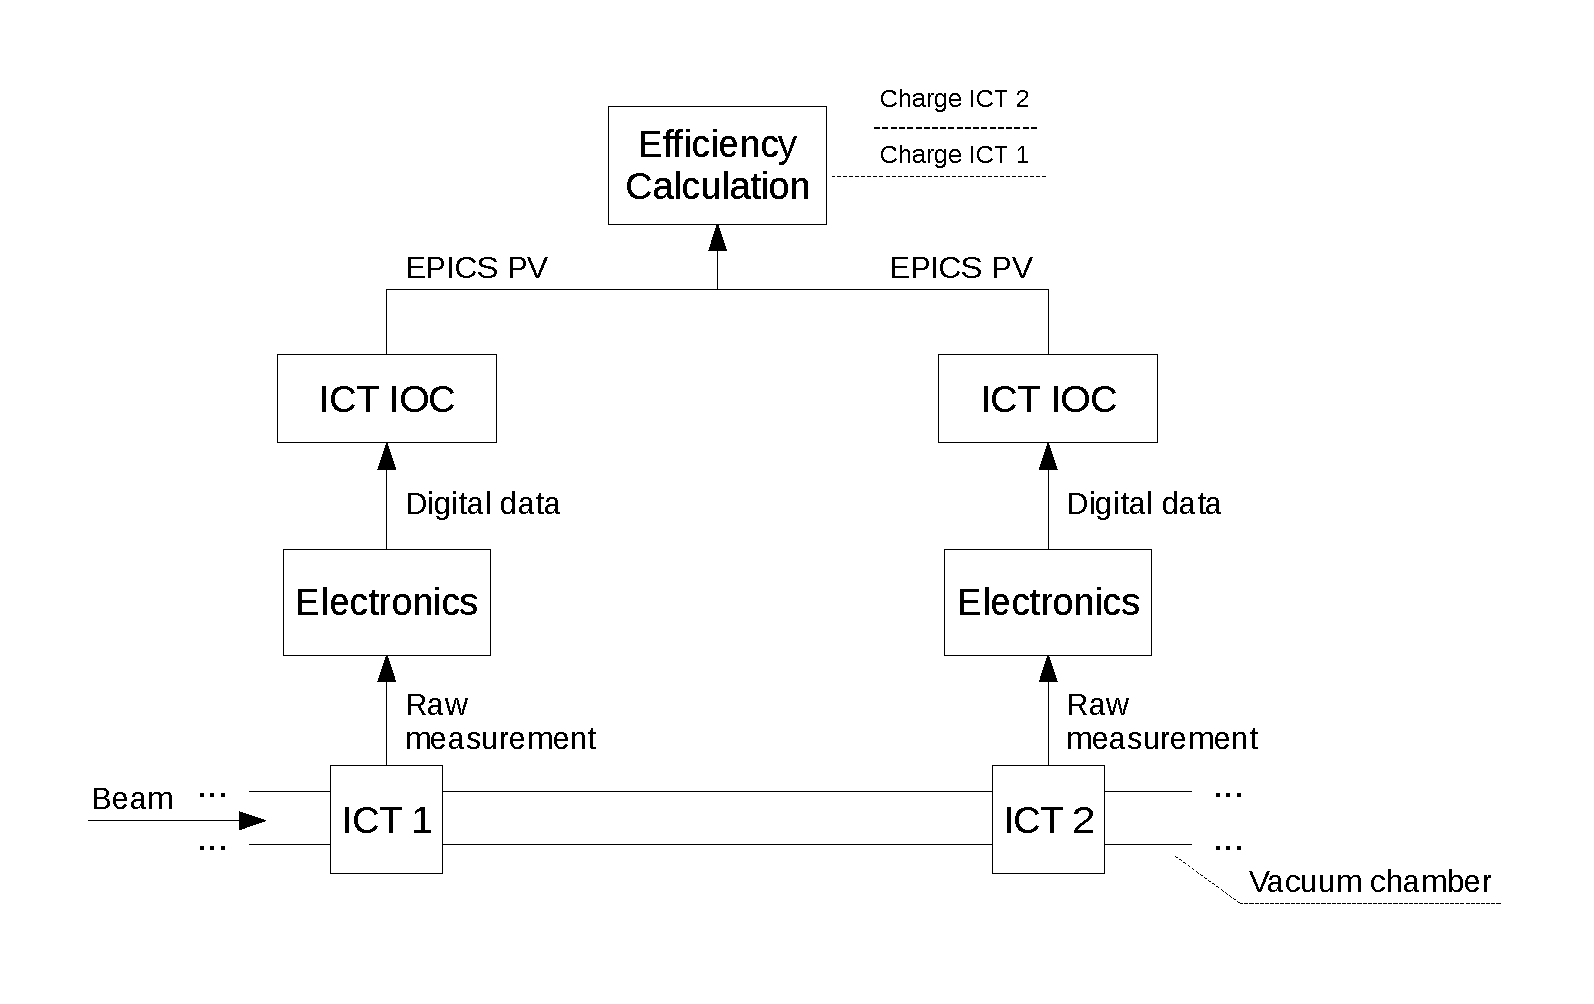
\includegraphics[width=1.0\textwidth]{eff-calc-overview-image}
	\end{figure}
\FloatBarrier

	\paragraph{} In order for the efficiency calculation to be consistent, it is necessary that both charge measurement values be updated and correspond to the same injected beam, at the start and end of the accelerator section which is being analyzed. The calculation synchronization is achieved by waiting for both charge measurement PVs to be updated before triggering the calculation. When the same PV is updated twice before the other one has been updated at least once since the last calculation has taken place, the synchronization has been lost and the Injection Efficiency IOC will indicate this by incrementing an error counter. In addition, only the newest of the measurements done for the same sensor is kept, and the charge measurement corresponding to the other sensor, which is missing, keeps being monitored.

%--- Section: Installing the IOC ---
\section{Installing the IOC}

	\paragraph{} In order to install the IOC, from the IOC top directory execute "make install".

	\bigskip
	\fcolorbox{margincolor}{backcolor}{
		\begin{tabularx}{0.9\textwidth}{X}
			\emph{cd \textless TOP IOC DIRECTORY\textgreater} \\
			\emph{make install} \\
		\end{tabularx}
	}

%--- Section: Running the IOC ---
\section{Running the IOC}

\section{Process Variables Description}\label{sec:process-variables}

	% Process Variables description table
	\begin{longtable}{| m{3.0cm} m{4.5cm} m{7.0cm} |}
		\caption{Application Process Variables} \\ \hline
		\bfseries Name & \bfseries Data Type & \bfseries Description \label{tab:PV-description} \endfirsthead
		\caption{Application Process Variables} \\ \hline
		\bfseries Name & \bfseries Data Type & \bfseries Description \endhead \hline
		% --- row ---
		Eff-Mon & FLOAT: 32-bit & \begin{tabular}{@{}m{6cm}@{}}
	    					Injection efficiency monitor. This PV displays the result of the division of the charge measurement value obtained by the first ICT sensor by the value obtained by the second ICT sensor.
						\end{tabular} \\ \hline
		% --- row ---
		EffHstr-Mon & FLOAT[1000] & \begin{tabular}{@{}m{6cm}@{}}
	    					Injection efficiency history. This PV contains the last 1000 results obtained by the efficiency calculation.
						\end{tabular} \\ \hline
		% --- row ---
		ErrorCnt-Mon & FLOAT: 32-bit & \begin{tabular}{@{}m{6cm}@{}}
	    					Error counter. This PV contains the number of synchronization errors identified. The error counter is incremented whenever the measurement of one of the 2 ICT sensors updates twice before the other can update. In order to reset the count, set the \emph{ErrorRst-Cmd} PV to \emph{ON}.
						\end{tabular} \\ \hline
		% --- row ---
		ErrorRst-Cmd & BOOL: OFF, ON & \begin{tabular}{@{}m{6cm}@{}}
				      	  	Error counter reset. This PV resets the error counter to 0 and erases the received measurements when set to \emph{ON}.
					  \end{tabular} \\ \hline
		% --- row ---
		FlgICT1-Mon & BOOL: 0, 1 & \begin{tabular}{@{}m{6cm}@{}}
				      	  	ICT 1 new data flag. When new data from ICT 1 is available, this PV is set to 1. The PV value remains equal to 1 until new data from the other ICT sensor is available, in which case both flags are set to 0.
					  \end{tabular} \\ \hline
		% --- row ---
		FlgICT2-Mon & BOOL: 0, 1 & \begin{tabular}{@{}m{6cm}@{}}
				      	  	ICT 2 new data flag. When new data from ICT 2 is available, this PV is set to 1. The PV value remains equal to 1 until new data from the other ICT sensor is available, in which case both flags are set to 0.
					  \end{tabular} \\ \hline
	\end{longtable}

\end{document}
\grid
